% Created by tikzDevice version 0.12.6 on 2026-02-09 13:37:35
% !TEX encoding = UTF-8 Unicode
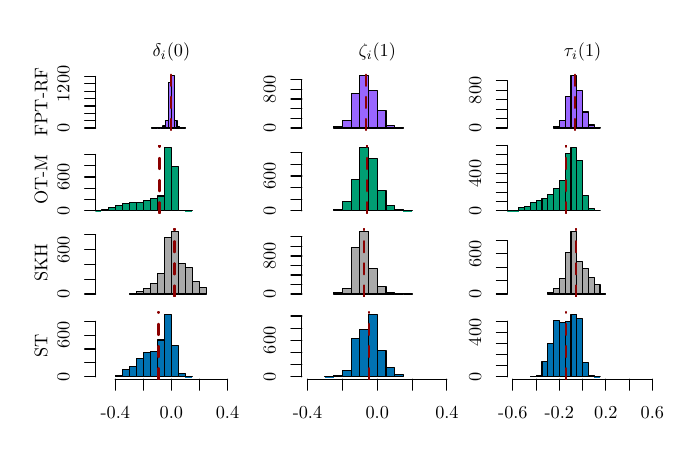
\begin{tikzpicture}[x=1pt,y=1pt]
\definecolor{fillColor}{RGB}{255,255,255}
\path[use as bounding box,fill=fillColor,fill opacity=0.00] (0,0) rectangle (230.90,143.67);
\begin{scope}
\path[clip] ( 24.55,106.66) rectangle ( 79.30,127.04);
\definecolor{drawColor}{RGB}{0,0,0}
\definecolor{fillColor}{RGB}{153,102,255}

\path[draw=drawColor,line width= 0.4pt,line join=round,line cap=round,fill=fillColor] ( 44.83,107.41) rectangle ( 45.84,107.43);

\path[draw=drawColor,line width= 0.4pt,line join=round,line cap=round,fill=fillColor] ( 45.84,107.41) rectangle ( 46.86,107.44);

\path[draw=drawColor,line width= 0.4pt,line join=round,line cap=round,fill=fillColor] ( 46.86,107.41) rectangle ( 47.87,107.47);

\path[draw=drawColor,line width= 0.4pt,line join=round,line cap=round,fill=fillColor] ( 47.87,107.41) rectangle ( 48.88,107.57);

\path[draw=drawColor,line width= 0.4pt,line join=round,line cap=round,fill=fillColor] ( 48.88,107.41) rectangle ( 49.90,108.13);

\path[draw=drawColor,line width= 0.4pt,line join=round,line cap=round,fill=fillColor] ( 49.90,107.41) rectangle ( 50.91,110.08);

\path[draw=drawColor,line width= 0.4pt,line join=round,line cap=round,fill=fillColor] ( 50.91,107.41) rectangle ( 51.92,123.75);

\path[draw=drawColor,line width= 0.4pt,line join=round,line cap=round,fill=fillColor] ( 51.92,107.41) rectangle ( 52.94,126.29);

\path[draw=drawColor,line width= 0.4pt,line join=round,line cap=round,fill=fillColor] ( 52.94,107.41) rectangle ( 53.95,110.22);

\path[draw=drawColor,line width= 0.4pt,line join=round,line cap=round,fill=fillColor] ( 53.95,107.41) rectangle ( 54.97,107.80);

\path[draw=drawColor,line width= 0.4pt,line join=round,line cap=round,fill=fillColor] ( 54.97,107.41) rectangle ( 55.98,107.48);

\path[draw=drawColor,line width= 0.4pt,line join=round,line cap=round,fill=fillColor] ( 55.98,107.41) rectangle ( 56.99,107.48);
\end{scope}
\begin{scope}
\path[clip] (  0.00,  0.00) rectangle (230.90,143.67);
\definecolor{drawColor}{RGB}{0,0,0}

\path[draw=drawColor,line width= 0.4pt,line join=round,line cap=round] ( 24.55,107.41) -- ( 24.55,126.01);

\path[draw=drawColor,line width= 0.4pt,line join=round,line cap=round] ( 24.55,107.41) -- ( 20.59,107.41);

\path[draw=drawColor,line width= 0.4pt,line join=round,line cap=round] ( 24.55,110.07) -- ( 20.59,110.07);

\path[draw=drawColor,line width= 0.4pt,line join=round,line cap=round] ( 24.55,112.73) -- ( 20.59,112.73);

\path[draw=drawColor,line width= 0.4pt,line join=round,line cap=round] ( 24.55,115.38) -- ( 20.59,115.38);

\path[draw=drawColor,line width= 0.4pt,line join=round,line cap=round] ( 24.55,118.04) -- ( 20.59,118.04);

\path[draw=drawColor,line width= 0.4pt,line join=round,line cap=round] ( 24.55,120.69) -- ( 20.59,120.69);

\path[draw=drawColor,line width= 0.4pt,line join=round,line cap=round] ( 24.55,123.35) -- ( 20.59,123.35);

\path[draw=drawColor,line width= 0.4pt,line join=round,line cap=round] ( 24.55,126.01) -- ( 20.59,126.01);

\node[text=drawColor,rotate= 90.00,anchor=base,inner sep=0pt, outer sep=0pt, scale=  0.66] at ( 15.05,107.41) {0};

\node[text=drawColor,rotate= 90.00,anchor=base,inner sep=0pt, outer sep=0pt, scale=  0.66] at ( 15.05,123.35) {1200};
\end{scope}
\begin{scope}
\path[clip] (  0.00,101.91) rectangle ( 82.47,143.67);
\definecolor{drawColor}{RGB}{0,0,0}

\node[text=drawColor,anchor=base,inner sep=0pt, outer sep=0pt, scale=  0.66] at ( 51.92,133.08) {\bfseries $\delta_i(0)$};

\node[text=drawColor,rotate= 90.00,anchor=base,inner sep=0pt, outer sep=0pt, scale=  0.66] at (  7.13,116.85) {FPT-RF};
\end{scope}
\begin{scope}
\path[clip] ( 24.55,106.66) rectangle ( 79.30,127.04);
\definecolor{drawColor}{RGB}{139,0,0}

\path[draw=drawColor,line width= 0.8pt,dash pattern=on 4pt off 4pt ,line join=round,line cap=round] ( 51.92,106.66) -- ( 51.92,127.04);
\end{scope}
\begin{scope}
\path[clip] ( 99.10,106.66) rectangle (153.52,127.04);
\definecolor{drawColor}{RGB}{0,0,0}
\definecolor{fillColor}{RGB}{153,102,255}

\path[draw=drawColor,line width= 0.4pt,line join=round,line cap=round,fill=fillColor] (110.56,107.41) rectangle (113.71,107.90);

\path[draw=drawColor,line width= 0.4pt,line join=round,line cap=round,fill=fillColor] (113.71,107.41) rectangle (116.86,110.26);

\path[draw=drawColor,line width= 0.4pt,line join=round,line cap=round,fill=fillColor] (116.86,107.41) rectangle (120.01,119.81);

\path[draw=drawColor,line width= 0.4pt,line join=round,line cap=round,fill=fillColor] (120.01,107.41) rectangle (123.16,126.29);

\path[draw=drawColor,line width= 0.4pt,line join=round,line cap=round,fill=fillColor] (123.16,107.41) rectangle (126.31,120.91);

\path[draw=drawColor,line width= 0.4pt,line join=round,line cap=round,fill=fillColor] (126.31,107.41) rectangle (129.46,113.65);

\path[draw=drawColor,line width= 0.4pt,line join=round,line cap=round,fill=fillColor] (129.46,107.41) rectangle (132.61,108.23);

\path[draw=drawColor,line width= 0.4pt,line join=round,line cap=round,fill=fillColor] (132.61,107.41) rectangle (135.75,107.69);
\end{scope}
\begin{scope}
\path[clip] (  0.00,  0.00) rectangle (230.90,143.67);
\definecolor{drawColor}{RGB}{0,0,0}

\path[draw=drawColor,line width= 0.4pt,line join=round,line cap=round] ( 99.10,107.41) -- ( 99.10,124.87);

\path[draw=drawColor,line width= 0.4pt,line join=round,line cap=round] ( 99.10,107.41) -- ( 95.14,107.41);

\path[draw=drawColor,line width= 0.4pt,line join=round,line cap=round] ( 99.10,110.91) -- ( 95.14,110.91);

\path[draw=drawColor,line width= 0.4pt,line join=round,line cap=round] ( 99.10,114.40) -- ( 95.14,114.40);

\path[draw=drawColor,line width= 0.4pt,line join=round,line cap=round] ( 99.10,117.89) -- ( 95.14,117.89);

\path[draw=drawColor,line width= 0.4pt,line join=round,line cap=round] ( 99.10,121.38) -- ( 95.14,121.38);

\path[draw=drawColor,line width= 0.4pt,line join=round,line cap=round] ( 99.10,124.87) -- ( 95.14,124.87);

\node[text=drawColor,rotate= 90.00,anchor=base,inner sep=0pt, outer sep=0pt, scale=  0.66] at ( 89.59,107.41) {0};

\node[text=drawColor,rotate= 90.00,anchor=base,inner sep=0pt, outer sep=0pt, scale=  0.66] at ( 89.59,121.38) {800};
\end{scope}
\begin{scope}
\path[clip] ( 82.47,101.91) rectangle (156.68,143.67);
\definecolor{drawColor}{RGB}{0,0,0}

\node[text=drawColor,anchor=base,inner sep=0pt, outer sep=0pt, scale=  0.66] at (126.31,133.08) {\bfseries $\zeta_i(1)$};
\end{scope}
\begin{scope}
\path[clip] ( 99.10,106.66) rectangle (153.52,127.04);
\definecolor{drawColor}{RGB}{139,0,0}

\path[draw=drawColor,line width= 0.8pt,dash pattern=on 4pt off 4pt ,line join=round,line cap=round] (122.20,106.66) -- (122.20,127.04);
\end{scope}
\begin{scope}
\path[clip] (173.32,106.66) rectangle (227.73,127.04);
\definecolor{drawColor}{RGB}{0,0,0}
\definecolor{fillColor}{RGB}{153,102,255}

\path[draw=drawColor,line width= 0.4pt,line join=round,line cap=round,fill=fillColor] (190.03,107.41) rectangle (192.13,107.86);

\path[draw=drawColor,line width= 0.4pt,line join=round,line cap=round,fill=fillColor] (192.13,107.41) rectangle (194.23,110.24);

\path[draw=drawColor,line width= 0.4pt,line join=round,line cap=round,fill=fillColor] (194.23,107.41) rectangle (196.33,118.86);

\path[draw=drawColor,line width= 0.4pt,line join=round,line cap=round,fill=fillColor] (196.33,107.41) rectangle (198.43,126.29);

\path[draw=drawColor,line width= 0.4pt,line join=round,line cap=round,fill=fillColor] (198.43,107.41) rectangle (200.53,120.85);

\path[draw=drawColor,line width= 0.4pt,line join=round,line cap=round,fill=fillColor] (200.53,107.41) rectangle (202.62,113.19);

\path[draw=drawColor,line width= 0.4pt,line join=round,line cap=round,fill=fillColor] (202.62,107.41) rectangle (204.72,108.49);

\path[draw=drawColor,line width= 0.4pt,line join=round,line cap=round,fill=fillColor] (204.72,107.41) rectangle (206.82,107.62);
\end{scope}
\begin{scope}
\path[clip] (  0.00,  0.00) rectangle (230.90,143.67);
\definecolor{drawColor}{RGB}{0,0,0}

\path[draw=drawColor,line width= 0.4pt,line join=round,line cap=round] (173.32,107.41) -- (173.32,124.45);

\path[draw=drawColor,line width= 0.4pt,line join=round,line cap=round] (173.32,107.41) -- (169.36,107.41);

\path[draw=drawColor,line width= 0.4pt,line join=round,line cap=round] (173.32,110.82) -- (169.36,110.82);

\path[draw=drawColor,line width= 0.4pt,line join=round,line cap=round] (173.32,114.23) -- (169.36,114.23);

\path[draw=drawColor,line width= 0.4pt,line join=round,line cap=round] (173.32,117.63) -- (169.36,117.63);

\path[draw=drawColor,line width= 0.4pt,line join=round,line cap=round] (173.32,121.04) -- (169.36,121.04);

\path[draw=drawColor,line width= 0.4pt,line join=round,line cap=round] (173.32,124.45) -- (169.36,124.45);

\node[text=drawColor,rotate= 90.00,anchor=base,inner sep=0pt, outer sep=0pt, scale=  0.66] at (163.81,107.41) {0};

\node[text=drawColor,rotate= 90.00,anchor=base,inner sep=0pt, outer sep=0pt, scale=  0.66] at (163.81,121.04) {800};
\end{scope}
\begin{scope}
\path[clip] (156.68,101.91) rectangle (230.90,143.67);
\definecolor{drawColor}{RGB}{0,0,0}

\node[text=drawColor,anchor=base,inner sep=0pt, outer sep=0pt, scale=  0.66] at (200.53,133.08) {\bfseries $\tau_i(1)$};
\end{scope}
\begin{scope}
\path[clip] (173.32,106.66) rectangle (227.73,127.04);
\definecolor{drawColor}{RGB}{139,0,0}

\path[draw=drawColor,line width= 0.8pt,dash pattern=on 4pt off 4pt ,line join=round,line cap=round] (197.79,106.66) -- (197.79,127.04);
\end{scope}
\begin{scope}
\path[clip] ( 24.55, 76.59) rectangle ( 79.30,101.12);
\definecolor{drawColor}{RGB}{0,0,0}
\definecolor{fillColor}{RGB}{0,158,115}

\path[draw=drawColor,line width= 0.4pt,line join=round,line cap=round,fill=fillColor] ( 21.51, 77.50) rectangle ( 24.05, 77.52);

\path[draw=drawColor,line width= 0.4pt,line join=round,line cap=round,fill=fillColor] ( 24.05, 77.50) rectangle ( 26.58, 77.52);

\path[draw=drawColor,line width= 0.4pt,line join=round,line cap=round,fill=fillColor] ( 26.58, 77.50) rectangle ( 29.11, 77.78);

\path[draw=drawColor,line width= 0.4pt,line join=round,line cap=round,fill=fillColor] ( 29.11, 77.50) rectangle ( 31.65, 78.66);

\path[draw=drawColor,line width= 0.4pt,line join=round,line cap=round,fill=fillColor] ( 31.65, 77.50) rectangle ( 34.18, 79.41);

\path[draw=drawColor,line width= 0.4pt,line join=round,line cap=round,fill=fillColor] ( 34.18, 77.50) rectangle ( 36.72, 80.04);

\path[draw=drawColor,line width= 0.4pt,line join=round,line cap=round,fill=fillColor] ( 36.72, 77.50) rectangle ( 39.25, 80.57);

\path[draw=drawColor,line width= 0.4pt,line join=round,line cap=round,fill=fillColor] ( 39.25, 77.50) rectangle ( 41.79, 80.65);

\path[draw=drawColor,line width= 0.4pt,line join=round,line cap=round,fill=fillColor] ( 41.79, 77.50) rectangle ( 44.32, 81.24);

\path[draw=drawColor,line width= 0.4pt,line join=round,line cap=round,fill=fillColor] ( 44.32, 77.50) rectangle ( 46.86, 81.93);

\path[draw=drawColor,line width= 0.4pt,line join=round,line cap=round,fill=fillColor] ( 46.86, 77.50) rectangle ( 49.39, 82.84);

\path[draw=drawColor,line width= 0.4pt,line join=round,line cap=round,fill=fillColor] ( 49.39, 77.50) rectangle ( 51.92,100.21);

\path[draw=drawColor,line width= 0.4pt,line join=round,line cap=round,fill=fillColor] ( 51.92, 77.50) rectangle ( 54.46, 93.42);

\path[draw=drawColor,line width= 0.4pt,line join=round,line cap=round,fill=fillColor] ( 54.46, 77.50) rectangle ( 56.99, 77.72);

\path[draw=drawColor,line width= 0.4pt,line join=round,line cap=round,fill=fillColor] ( 56.99, 77.50) rectangle ( 59.53, 77.52);
\end{scope}
\begin{scope}
\path[clip] (  0.00,  0.00) rectangle (230.90,143.67);
\definecolor{drawColor}{RGB}{0,0,0}

\path[draw=drawColor,line width= 0.4pt,line join=round,line cap=round] ( 24.55, 77.50) -- ( 24.55, 97.83);

\path[draw=drawColor,line width= 0.4pt,line join=round,line cap=round] ( 24.55, 77.50) -- ( 20.59, 77.50);

\path[draw=drawColor,line width= 0.4pt,line join=round,line cap=round] ( 24.55, 81.56) -- ( 20.59, 81.56);

\path[draw=drawColor,line width= 0.4pt,line join=round,line cap=round] ( 24.55, 85.63) -- ( 20.59, 85.63);

\path[draw=drawColor,line width= 0.4pt,line join=round,line cap=round] ( 24.55, 89.70) -- ( 20.59, 89.70);

\path[draw=drawColor,line width= 0.4pt,line join=round,line cap=round] ( 24.55, 93.76) -- ( 20.59, 93.76);

\path[draw=drawColor,line width= 0.4pt,line join=round,line cap=round] ( 24.55, 97.83) -- ( 20.59, 97.83);

\node[text=drawColor,rotate= 90.00,anchor=base,inner sep=0pt, outer sep=0pt, scale=  0.66] at ( 15.05, 77.50) {0};

\node[text=drawColor,rotate= 90.00,anchor=base,inner sep=0pt, outer sep=0pt, scale=  0.66] at ( 15.05, 89.70) {600};
\end{scope}
\begin{scope}
\path[clip] (  0.00, 71.84) rectangle ( 82.47,101.91);
\definecolor{drawColor}{RGB}{0,0,0}

\node[text=drawColor,rotate= 90.00,anchor=base,inner sep=0pt, outer sep=0pt, scale=  0.66] at (  7.13, 88.85) {OT-M};
\end{scope}
\begin{scope}
\path[clip] ( 24.55, 76.59) rectangle ( 79.30,101.12);
\definecolor{drawColor}{RGB}{139,0,0}

\path[draw=drawColor,line width= 0.8pt,dash pattern=on 4pt off 4pt ,line join=round,line cap=round] ( 47.62, 76.59) -- ( 47.62,101.12);
\end{scope}
\begin{scope}
\path[clip] ( 99.10, 76.59) rectangle (153.52,101.12);
\definecolor{drawColor}{RGB}{0,0,0}
\definecolor{fillColor}{RGB}{0,158,115}

\path[draw=drawColor,line width= 0.4pt,line join=round,line cap=round,fill=fillColor] (110.56, 77.50) rectangle (113.71, 77.98);

\path[draw=drawColor,line width= 0.4pt,line join=round,line cap=round,fill=fillColor] (113.71, 77.50) rectangle (116.86, 80.86);

\path[draw=drawColor,line width= 0.4pt,line join=round,line cap=round,fill=fillColor] (116.86, 77.50) rectangle (120.01, 88.91);

\path[draw=drawColor,line width= 0.4pt,line join=round,line cap=round,fill=fillColor] (120.01, 77.50) rectangle (123.16,100.21);

\path[draw=drawColor,line width= 0.4pt,line join=round,line cap=round,fill=fillColor] (123.16, 77.50) rectangle (126.31, 96.47);

\path[draw=drawColor,line width= 0.4pt,line join=round,line cap=round,fill=fillColor] (126.31, 77.50) rectangle (129.46, 84.88);

\path[draw=drawColor,line width= 0.4pt,line join=round,line cap=round,fill=fillColor] (129.46, 77.50) rectangle (132.61, 79.43);

\path[draw=drawColor,line width= 0.4pt,line join=round,line cap=round,fill=fillColor] (132.61, 77.50) rectangle (135.75, 77.83);

\path[draw=drawColor,line width= 0.4pt,line join=round,line cap=round,fill=fillColor] (135.75, 77.50) rectangle (138.90, 77.54);
\end{scope}
\begin{scope}
\path[clip] (  0.00,  0.00) rectangle (230.90,143.67);
\definecolor{drawColor}{RGB}{0,0,0}

\path[draw=drawColor,line width= 0.4pt,line join=round,line cap=round] ( 99.10, 77.50) -- ( 99.10, 98.49);

\path[draw=drawColor,line width= 0.4pt,line join=round,line cap=round] ( 99.10, 77.50) -- ( 95.14, 77.50);

\path[draw=drawColor,line width= 0.4pt,line join=round,line cap=round] ( 99.10, 81.69) -- ( 95.14, 81.69);

\path[draw=drawColor,line width= 0.4pt,line join=round,line cap=round] ( 99.10, 85.89) -- ( 95.14, 85.89);

\path[draw=drawColor,line width= 0.4pt,line join=round,line cap=round] ( 99.10, 90.09) -- ( 95.14, 90.09);

\path[draw=drawColor,line width= 0.4pt,line join=round,line cap=round] ( 99.10, 94.29) -- ( 95.14, 94.29);

\path[draw=drawColor,line width= 0.4pt,line join=round,line cap=round] ( 99.10, 98.49) -- ( 95.14, 98.49);

\node[text=drawColor,rotate= 90.00,anchor=base,inner sep=0pt, outer sep=0pt, scale=  0.66] at ( 89.59, 77.50) {0};

\node[text=drawColor,rotate= 90.00,anchor=base,inner sep=0pt, outer sep=0pt, scale=  0.66] at ( 89.59, 90.09) {600};
\end{scope}
\begin{scope}
\path[clip] ( 99.10, 76.59) rectangle (153.52,101.12);
\definecolor{drawColor}{RGB}{139,0,0}

\path[draw=drawColor,line width= 0.8pt,dash pattern=on 4pt off 4pt ,line join=round,line cap=round] (122.64, 76.59) -- (122.64,101.12);
\end{scope}
\begin{scope}
\path[clip] (173.32, 76.59) rectangle (227.73,101.12);
\definecolor{drawColor}{RGB}{0,0,0}
\definecolor{fillColor}{RGB}{0,158,115}

\path[draw=drawColor,line width= 0.4pt,line join=round,line cap=round,fill=fillColor] (173.23, 77.50) rectangle (175.33, 77.53);

\path[draw=drawColor,line width= 0.4pt,line join=round,line cap=round,fill=fillColor] (175.33, 77.50) rectangle (177.43, 77.60);

\path[draw=drawColor,line width= 0.4pt,line join=round,line cap=round,fill=fillColor] (177.43, 77.50) rectangle (179.53, 78.64);

\path[draw=drawColor,line width= 0.4pt,line join=round,line cap=round,fill=fillColor] (179.53, 77.50) rectangle (181.63, 79.08);

\path[draw=drawColor,line width= 0.4pt,line join=round,line cap=round,fill=fillColor] (181.63, 77.50) rectangle (183.73, 80.43);

\path[draw=drawColor,line width= 0.4pt,line join=round,line cap=round,fill=fillColor] (183.73, 77.50) rectangle (185.83, 81.17);

\path[draw=drawColor,line width= 0.4pt,line join=round,line cap=round,fill=fillColor] (185.83, 77.50) rectangle (187.93, 81.88);

\path[draw=drawColor,line width= 0.4pt,line join=round,line cap=round,fill=fillColor] (187.93, 77.50) rectangle (190.03, 83.46);

\path[draw=drawColor,line width= 0.4pt,line join=round,line cap=round,fill=fillColor] (190.03, 77.50) rectangle (192.13, 85.55);

\path[draw=drawColor,line width= 0.4pt,line join=round,line cap=round,fill=fillColor] (192.13, 77.50) rectangle (194.23, 88.41);

\path[draw=drawColor,line width= 0.4pt,line join=round,line cap=round,fill=fillColor] (194.23, 77.50) rectangle (196.33, 98.08);

\path[draw=drawColor,line width= 0.4pt,line join=round,line cap=round,fill=fillColor] (196.33, 77.50) rectangle (198.43,100.21);

\path[draw=drawColor,line width= 0.4pt,line join=round,line cap=round,fill=fillColor] (198.43, 77.50) rectangle (200.53, 95.79);

\path[draw=drawColor,line width= 0.4pt,line join=round,line cap=round,fill=fillColor] (200.53, 77.50) rectangle (202.62, 83.06);

\path[draw=drawColor,line width= 0.4pt,line join=round,line cap=round,fill=fillColor] (202.62, 77.50) rectangle (204.72, 78.37);

\path[draw=drawColor,line width= 0.4pt,line join=round,line cap=round,fill=fillColor] (204.72, 77.50) rectangle (206.82, 77.67);
\end{scope}
\begin{scope}
\path[clip] (  0.00,  0.00) rectangle (230.90,143.67);
\definecolor{drawColor}{RGB}{0,0,0}

\path[draw=drawColor,line width= 0.4pt,line join=round,line cap=round] (173.32, 77.50) -- (173.32,101.08);

\path[draw=drawColor,line width= 0.4pt,line join=round,line cap=round] (173.32, 77.50) -- (169.36, 77.50);

\path[draw=drawColor,line width= 0.4pt,line join=round,line cap=round] (173.32, 80.87) -- (169.36, 80.87);

\path[draw=drawColor,line width= 0.4pt,line join=round,line cap=round] (173.32, 84.24) -- (169.36, 84.24);

\path[draw=drawColor,line width= 0.4pt,line join=round,line cap=round] (173.32, 87.61) -- (169.36, 87.61);

\path[draw=drawColor,line width= 0.4pt,line join=round,line cap=round] (173.32, 90.97) -- (169.36, 90.97);

\path[draw=drawColor,line width= 0.4pt,line join=round,line cap=round] (173.32, 94.34) -- (169.36, 94.34);

\path[draw=drawColor,line width= 0.4pt,line join=round,line cap=round] (173.32, 97.71) -- (169.36, 97.71);

\path[draw=drawColor,line width= 0.4pt,line join=round,line cap=round] (173.32,101.08) -- (169.36,101.08);

\node[text=drawColor,rotate= 90.00,anchor=base,inner sep=0pt, outer sep=0pt, scale=  0.66] at (163.81, 77.50) {0};

\node[text=drawColor,rotate= 90.00,anchor=base,inner sep=0pt, outer sep=0pt, scale=  0.66] at (163.81, 90.97) {400};
\end{scope}
\begin{scope}
\path[clip] (173.32, 76.59) rectangle (227.73,101.12);
\definecolor{drawColor}{RGB}{139,0,0}

\path[draw=drawColor,line width= 0.8pt,dash pattern=on 4pt off 4pt ,line join=round,line cap=round] (194.51, 76.59) -- (194.51,101.12);
\end{scope}
\begin{scope}
\path[clip] ( 24.55, 46.52) rectangle ( 79.30, 71.04);
\definecolor{drawColor}{RGB}{0,0,0}
\definecolor{fillColor}{RGB}{169,169,169}

\path[draw=drawColor,line width= 0.4pt,line join=round,line cap=round,fill=fillColor] ( 36.72, 47.43) rectangle ( 39.25, 47.45);

\path[draw=drawColor,line width= 0.4pt,line join=round,line cap=round,fill=fillColor] ( 39.25, 47.43) rectangle ( 41.79, 48.31);

\path[draw=drawColor,line width= 0.4pt,line join=round,line cap=round,fill=fillColor] ( 41.79, 47.43) rectangle ( 44.32, 49.54);

\path[draw=drawColor,line width= 0.4pt,line join=round,line cap=round,fill=fillColor] ( 44.32, 47.43) rectangle ( 46.86, 51.14);

\path[draw=drawColor,line width= 0.4pt,line join=round,line cap=round,fill=fillColor] ( 46.86, 47.43) rectangle ( 49.39, 54.93);

\path[draw=drawColor,line width= 0.4pt,line join=round,line cap=round,fill=fillColor] ( 49.39, 47.43) rectangle ( 51.92, 67.70);

\path[draw=drawColor,line width= 0.4pt,line join=round,line cap=round,fill=fillColor] ( 51.92, 47.43) rectangle ( 54.46, 70.14);

\path[draw=drawColor,line width= 0.4pt,line join=round,line cap=round,fill=fillColor] ( 54.46, 47.43) rectangle ( 56.99, 58.35);

\path[draw=drawColor,line width= 0.4pt,line join=round,line cap=round,fill=fillColor] ( 56.99, 47.43) rectangle ( 59.53, 57.10);

\path[draw=drawColor,line width= 0.4pt,line join=round,line cap=round,fill=fillColor] ( 59.53, 47.43) rectangle ( 62.06, 52.05);

\path[draw=drawColor,line width= 0.4pt,line join=round,line cap=round,fill=fillColor] ( 62.06, 47.43) rectangle ( 64.60, 49.80);
\end{scope}
\begin{scope}
\path[clip] (  0.00,  0.00) rectangle (230.90,143.67);
\definecolor{drawColor}{RGB}{0,0,0}

\path[draw=drawColor,line width= 0.4pt,line join=round,line cap=round] ( 24.55, 47.43) -- ( 24.55, 68.80);

\path[draw=drawColor,line width= 0.4pt,line join=round,line cap=round] ( 24.55, 47.43) -- ( 20.59, 47.43);

\path[draw=drawColor,line width= 0.4pt,line join=round,line cap=round] ( 24.55, 52.77) -- ( 20.59, 52.77);

\path[draw=drawColor,line width= 0.4pt,line join=round,line cap=round] ( 24.55, 58.11) -- ( 20.59, 58.11);

\path[draw=drawColor,line width= 0.4pt,line join=round,line cap=round] ( 24.55, 63.46) -- ( 20.59, 63.46);

\path[draw=drawColor,line width= 0.4pt,line join=round,line cap=round] ( 24.55, 68.80) -- ( 20.59, 68.80);

\node[text=drawColor,rotate= 90.00,anchor=base,inner sep=0pt, outer sep=0pt, scale=  0.66] at ( 15.05, 47.43) {0};

\node[text=drawColor,rotate= 90.00,anchor=base,inner sep=0pt, outer sep=0pt, scale=  0.66] at ( 15.05, 63.46) {600};
\end{scope}
\begin{scope}
\path[clip] (  0.00, 41.77) rectangle ( 82.47, 71.84);
\definecolor{drawColor}{RGB}{0,0,0}

\node[text=drawColor,rotate= 90.00,anchor=base,inner sep=0pt, outer sep=0pt, scale=  0.66] at (  7.13, 58.78) {SKH};
\end{scope}
\begin{scope}
\path[clip] ( 24.55, 46.52) rectangle ( 79.30, 71.04);
\definecolor{drawColor}{RGB}{139,0,0}

\path[draw=drawColor,line width= 0.8pt,dash pattern=on 4pt off 4pt ,line join=round,line cap=round] ( 53.02, 46.52) -- ( 53.02, 71.04);
\end{scope}
\begin{scope}
\path[clip] ( 99.10, 46.52) rectangle (153.52, 71.04);
\definecolor{drawColor}{RGB}{0,0,0}
\definecolor{fillColor}{RGB}{169,169,169}

\path[draw=drawColor,line width= 0.4pt,line join=round,line cap=round,fill=fillColor] (110.56, 47.43) rectangle (113.71, 47.87);

\path[draw=drawColor,line width= 0.4pt,line join=round,line cap=round,fill=fillColor] (113.71, 47.43) rectangle (116.86, 49.37);

\path[draw=drawColor,line width= 0.4pt,line join=round,line cap=round,fill=fillColor] (116.86, 47.43) rectangle (120.01, 64.24);

\path[draw=drawColor,line width= 0.4pt,line join=round,line cap=round,fill=fillColor] (120.01, 47.43) rectangle (123.16, 70.14);

\path[draw=drawColor,line width= 0.4pt,line join=round,line cap=round,fill=fillColor] (123.16, 47.43) rectangle (126.31, 56.80);

\path[draw=drawColor,line width= 0.4pt,line join=round,line cap=round,fill=fillColor] (126.31, 47.43) rectangle (129.46, 50.07);

\path[draw=drawColor,line width= 0.4pt,line join=round,line cap=round,fill=fillColor] (129.46, 47.43) rectangle (132.61, 47.86);

\path[draw=drawColor,line width= 0.4pt,line join=round,line cap=round,fill=fillColor] (132.61, 47.43) rectangle (135.75, 47.63);

\path[draw=drawColor,line width= 0.4pt,line join=round,line cap=round,fill=fillColor] (135.75, 47.43) rectangle (138.90, 47.44);
\end{scope}
\begin{scope}
\path[clip] (  0.00,  0.00) rectangle (230.90,143.67);
\definecolor{drawColor}{RGB}{0,0,0}

\path[draw=drawColor,line width= 0.4pt,line join=round,line cap=round] ( 99.10, 47.43) -- ( 99.10, 68.06);

\path[draw=drawColor,line width= 0.4pt,line join=round,line cap=round] ( 99.10, 47.43) -- ( 95.14, 47.43);

\path[draw=drawColor,line width= 0.4pt,line join=round,line cap=round] ( 99.10, 50.86) -- ( 95.14, 50.86);

\path[draw=drawColor,line width= 0.4pt,line join=round,line cap=round] ( 99.10, 54.30) -- ( 95.14, 54.30);

\path[draw=drawColor,line width= 0.4pt,line join=round,line cap=round] ( 99.10, 57.74) -- ( 95.14, 57.74);

\path[draw=drawColor,line width= 0.4pt,line join=round,line cap=round] ( 99.10, 61.18) -- ( 95.14, 61.18);

\path[draw=drawColor,line width= 0.4pt,line join=round,line cap=round] ( 99.10, 64.62) -- ( 95.14, 64.62);

\path[draw=drawColor,line width= 0.4pt,line join=round,line cap=round] ( 99.10, 68.06) -- ( 95.14, 68.06);

\node[text=drawColor,rotate= 90.00,anchor=base,inner sep=0pt, outer sep=0pt, scale=  0.66] at ( 89.59, 47.43) {0};

\node[text=drawColor,rotate= 90.00,anchor=base,inner sep=0pt, outer sep=0pt, scale=  0.66] at ( 89.59, 61.18) {800};
\end{scope}
\begin{scope}
\path[clip] ( 99.10, 46.52) rectangle (153.52, 71.04);
\definecolor{drawColor}{RGB}{139,0,0}

\path[draw=drawColor,line width= 0.8pt,dash pattern=on 4pt off 4pt ,line join=round,line cap=round] (121.39, 46.52) -- (121.39, 71.04);
\end{scope}
\begin{scope}
\path[clip] (173.32, 46.52) rectangle (227.73, 71.04);
\definecolor{drawColor}{RGB}{0,0,0}
\definecolor{fillColor}{RGB}{169,169,169}

\path[draw=drawColor,line width= 0.4pt,line join=round,line cap=round,fill=fillColor] (187.93, 47.43) rectangle (190.03, 47.91);

\path[draw=drawColor,line width= 0.4pt,line join=round,line cap=round,fill=fillColor] (190.03, 47.43) rectangle (192.13, 49.55);

\path[draw=drawColor,line width= 0.4pt,line join=round,line cap=round,fill=fillColor] (192.13, 47.43) rectangle (194.23, 53.05);

\path[draw=drawColor,line width= 0.4pt,line join=round,line cap=round,fill=fillColor] (194.23, 47.43) rectangle (196.33, 62.36);

\path[draw=drawColor,line width= 0.4pt,line join=round,line cap=round,fill=fillColor] (196.33, 47.43) rectangle (198.43, 70.14);

\path[draw=drawColor,line width= 0.4pt,line join=round,line cap=round,fill=fillColor] (198.43, 47.43) rectangle (200.53, 59.15);

\path[draw=drawColor,line width= 0.4pt,line join=round,line cap=round,fill=fillColor] (200.53, 47.43) rectangle (202.62, 56.77);

\path[draw=drawColor,line width= 0.4pt,line join=round,line cap=round,fill=fillColor] (202.62, 47.43) rectangle (204.72, 53.48);

\path[draw=drawColor,line width= 0.4pt,line join=round,line cap=round,fill=fillColor] (204.72, 47.43) rectangle (206.82, 50.93);

\path[draw=drawColor,line width= 0.4pt,line join=round,line cap=round,fill=fillColor] (206.82, 47.43) rectangle (208.92, 47.55);
\end{scope}
\begin{scope}
\path[clip] (  0.00,  0.00) rectangle (230.90,143.67);
\definecolor{drawColor}{RGB}{0,0,0}

\path[draw=drawColor,line width= 0.4pt,line join=round,line cap=round] (173.32, 47.43) -- (173.32, 66.73);

\path[draw=drawColor,line width= 0.4pt,line join=round,line cap=round] (173.32, 47.43) -- (169.36, 47.43);

\path[draw=drawColor,line width= 0.4pt,line join=round,line cap=round] (173.32, 52.25) -- (169.36, 52.25);

\path[draw=drawColor,line width= 0.4pt,line join=round,line cap=round] (173.32, 57.08) -- (169.36, 57.08);

\path[draw=drawColor,line width= 0.4pt,line join=round,line cap=round] (173.32, 61.91) -- (169.36, 61.91);

\path[draw=drawColor,line width= 0.4pt,line join=round,line cap=round] (173.32, 66.73) -- (169.36, 66.73);

\node[text=drawColor,rotate= 90.00,anchor=base,inner sep=0pt, outer sep=0pt, scale=  0.66] at (163.81, 47.43) {0};

\node[text=drawColor,rotate= 90.00,anchor=base,inner sep=0pt, outer sep=0pt, scale=  0.66] at (163.81, 61.91) {600};
\end{scope}
\begin{scope}
\path[clip] (173.32, 46.52) rectangle (227.73, 71.04);
\definecolor{drawColor}{RGB}{139,0,0}

\path[draw=drawColor,line width= 0.8pt,dash pattern=on 4pt off 4pt ,line join=round,line cap=round] (198.16, 46.52) -- (198.16, 71.04);
\end{scope}
\begin{scope}
\path[clip] ( 24.55, 16.63) rectangle ( 79.30, 40.97);
\definecolor{drawColor}{RGB}{0,0,0}
\definecolor{fillColor}{RGB}{0,114,178}

\path[draw=drawColor,line width= 0.4pt,line join=round,line cap=round,fill=fillColor] ( 31.65, 17.53) rectangle ( 34.18, 17.98);

\path[draw=drawColor,line width= 0.4pt,line join=round,line cap=round,fill=fillColor] ( 34.18, 17.53) rectangle ( 36.72, 20.16);

\path[draw=drawColor,line width= 0.4pt,line join=round,line cap=round,fill=fillColor] ( 36.72, 17.53) rectangle ( 39.25, 21.19);

\path[draw=drawColor,line width= 0.4pt,line join=round,line cap=round,fill=fillColor] ( 39.25, 17.53) rectangle ( 41.79, 24.14);

\path[draw=drawColor,line width= 0.4pt,line join=round,line cap=round,fill=fillColor] ( 41.79, 17.53) rectangle ( 44.32, 26.30);

\path[draw=drawColor,line width= 0.4pt,line join=round,line cap=round,fill=fillColor] ( 44.32, 17.53) rectangle ( 46.86, 26.60);

\path[draw=drawColor,line width= 0.4pt,line join=round,line cap=round,fill=fillColor] ( 46.86, 17.53) rectangle ( 49.39, 30.81);

\path[draw=drawColor,line width= 0.4pt,line join=round,line cap=round,fill=fillColor] ( 49.39, 17.53) rectangle ( 51.92, 40.07);

\path[draw=drawColor,line width= 0.4pt,line join=round,line cap=round,fill=fillColor] ( 51.92, 17.53) rectangle ( 54.46, 28.95);

\path[draw=drawColor,line width= 0.4pt,line join=round,line cap=round,fill=fillColor] ( 54.46, 17.53) rectangle ( 56.99, 18.61);

\path[draw=drawColor,line width= 0.4pt,line join=round,line cap=round,fill=fillColor] ( 56.99, 17.53) rectangle ( 59.53, 17.56);
\end{scope}
\begin{scope}
\path[clip] (  0.00,  0.00) rectangle (230.90,143.67);
\definecolor{drawColor}{RGB}{0,0,0}

\path[draw=drawColor,line width= 0.4pt,line join=round,line cap=round] ( 31.65, 16.63) -- ( 72.20, 16.63);

\path[draw=drawColor,line width= 0.4pt,line join=round,line cap=round] ( 31.65, 16.63) -- ( 31.65, 12.67);

\path[draw=drawColor,line width= 0.4pt,line join=round,line cap=round] ( 41.79, 16.63) -- ( 41.79, 12.67);

\path[draw=drawColor,line width= 0.4pt,line join=round,line cap=round] ( 51.92, 16.63) -- ( 51.92, 12.67);

\path[draw=drawColor,line width= 0.4pt,line join=round,line cap=round] ( 62.06, 16.63) -- ( 62.06, 12.67);

\path[draw=drawColor,line width= 0.4pt,line join=round,line cap=round] ( 72.20, 16.63) -- ( 72.20, 12.67);

\node[text=drawColor,anchor=base,inner sep=0pt, outer sep=0pt, scale=  0.66] at ( 31.65,  2.38) {-0.4};

\node[text=drawColor,anchor=base,inner sep=0pt, outer sep=0pt, scale=  0.66] at ( 51.92,  2.38) {0.0};

\node[text=drawColor,anchor=base,inner sep=0pt, outer sep=0pt, scale=  0.66] at ( 72.20,  2.38) {0.4};

\path[draw=drawColor,line width= 0.4pt,line join=round,line cap=round] ( 24.55, 17.53) -- ( 24.55, 37.57);

\path[draw=drawColor,line width= 0.4pt,line join=round,line cap=round] ( 24.55, 17.53) -- ( 20.59, 17.53);

\path[draw=drawColor,line width= 0.4pt,line join=round,line cap=round] ( 24.55, 22.54) -- ( 20.59, 22.54);

\path[draw=drawColor,line width= 0.4pt,line join=round,line cap=round] ( 24.55, 27.55) -- ( 20.59, 27.55);

\path[draw=drawColor,line width= 0.4pt,line join=round,line cap=round] ( 24.55, 32.56) -- ( 20.59, 32.56);

\path[draw=drawColor,line width= 0.4pt,line join=round,line cap=round] ( 24.55, 37.57) -- ( 20.59, 37.57);

\node[text=drawColor,rotate= 90.00,anchor=base,inner sep=0pt, outer sep=0pt, scale=  0.66] at ( 15.05, 17.53) {0};

\node[text=drawColor,rotate= 90.00,anchor=base,inner sep=0pt, outer sep=0pt, scale=  0.66] at ( 15.05, 32.56) {600};
\end{scope}
\begin{scope}
\path[clip] (  0.00,  0.00) rectangle ( 82.47, 41.77);
\definecolor{drawColor}{RGB}{0,0,0}

\node[text=drawColor,rotate= 90.00,anchor=base,inner sep=0pt, outer sep=0pt, scale=  0.66] at (  7.13, 28.80) {ST};
\end{scope}
\begin{scope}
\path[clip] ( 24.55, 16.63) rectangle ( 79.30, 40.97);
\definecolor{drawColor}{RGB}{139,0,0}

\path[draw=drawColor,line width= 0.8pt,dash pattern=on 4pt off 4pt ,line join=round,line cap=round] ( 47.26, 16.63) -- ( 47.26, 40.97);
\end{scope}
\begin{scope}
\path[clip] ( 99.10, 16.63) rectangle (153.52, 40.97);
\definecolor{drawColor}{RGB}{0,0,0}
\definecolor{fillColor}{RGB}{0,114,178}

\path[draw=drawColor,line width= 0.4pt,line join=round,line cap=round,fill=fillColor] (107.41, 17.53) rectangle (110.56, 17.58);

\path[draw=drawColor,line width= 0.4pt,line join=round,line cap=round,fill=fillColor] (110.56, 17.53) rectangle (113.71, 17.84);

\path[draw=drawColor,line width= 0.4pt,line join=round,line cap=round,fill=fillColor] (113.71, 17.53) rectangle (116.86, 19.64);

\path[draw=drawColor,line width= 0.4pt,line join=round,line cap=round,fill=fillColor] (116.86, 17.53) rectangle (120.01, 31.36);

\path[draw=drawColor,line width= 0.4pt,line join=round,line cap=round,fill=fillColor] (120.01, 17.53) rectangle (123.16, 34.74);

\path[draw=drawColor,line width= 0.4pt,line join=round,line cap=round,fill=fillColor] (123.16, 17.53) rectangle (126.31, 40.07);

\path[draw=drawColor,line width= 0.4pt,line join=round,line cap=round,fill=fillColor] (126.31, 17.53) rectangle (129.46, 26.90);

\path[draw=drawColor,line width= 0.4pt,line join=round,line cap=round,fill=fillColor] (129.46, 17.53) rectangle (132.61, 20.85);

\path[draw=drawColor,line width= 0.4pt,line join=round,line cap=round,fill=fillColor] (132.61, 17.53) rectangle (135.75, 18.50);
\end{scope}
\begin{scope}
\path[clip] (  0.00,  0.00) rectangle (230.90,143.67);
\definecolor{drawColor}{RGB}{0,0,0}

\path[draw=drawColor,line width= 0.4pt,line join=round,line cap=round] (101.11, 16.63) -- (151.50, 16.63);

\path[draw=drawColor,line width= 0.4pt,line join=round,line cap=round] (101.11, 16.63) -- (101.11, 12.67);

\path[draw=drawColor,line width= 0.4pt,line join=round,line cap=round] (113.71, 16.63) -- (113.71, 12.67);

\path[draw=drawColor,line width= 0.4pt,line join=round,line cap=round] (126.31, 16.63) -- (126.31, 12.67);

\path[draw=drawColor,line width= 0.4pt,line join=round,line cap=round] (138.90, 16.63) -- (138.90, 12.67);

\path[draw=drawColor,line width= 0.4pt,line join=round,line cap=round] (151.50, 16.63) -- (151.50, 12.67);

\node[text=drawColor,anchor=base,inner sep=0pt, outer sep=0pt, scale=  0.66] at (101.11,  2.38) {-0.4};

\node[text=drawColor,anchor=base,inner sep=0pt, outer sep=0pt, scale=  0.66] at (126.31,  2.38) {0.0};

\node[text=drawColor,anchor=base,inner sep=0pt, outer sep=0pt, scale=  0.66] at (151.50,  2.38) {0.4};

\path[draw=drawColor,line width= 0.4pt,line join=round,line cap=round] ( 99.10, 17.53) -- ( 99.10, 39.48);

\path[draw=drawColor,line width= 0.4pt,line join=round,line cap=round] ( 99.10, 17.53) -- ( 95.14, 17.53);

\path[draw=drawColor,line width= 0.4pt,line join=round,line cap=round] ( 99.10, 21.92) -- ( 95.14, 21.92);

\path[draw=drawColor,line width= 0.4pt,line join=round,line cap=round] ( 99.10, 26.31) -- ( 95.14, 26.31);

\path[draw=drawColor,line width= 0.4pt,line join=round,line cap=round] ( 99.10, 30.70) -- ( 95.14, 30.70);

\path[draw=drawColor,line width= 0.4pt,line join=round,line cap=round] ( 99.10, 35.09) -- ( 95.14, 35.09);

\path[draw=drawColor,line width= 0.4pt,line join=round,line cap=round] ( 99.10, 39.48) -- ( 95.14, 39.48);

\node[text=drawColor,rotate= 90.00,anchor=base,inner sep=0pt, outer sep=0pt, scale=  0.66] at ( 89.59, 17.53) {0};

\node[text=drawColor,rotate= 90.00,anchor=base,inner sep=0pt, outer sep=0pt, scale=  0.66] at ( 89.59, 30.70) {600};
\end{scope}
\begin{scope}
\path[clip] ( 99.10, 16.63) rectangle (153.52, 40.97);
\definecolor{drawColor}{RGB}{139,0,0}

\path[draw=drawColor,line width= 0.8pt,dash pattern=on 4pt off 4pt ,line join=round,line cap=round] (123.20, 16.63) -- (123.20, 40.97);
\end{scope}
\begin{scope}
\path[clip] (173.32, 16.63) rectangle (227.73, 40.97);
\definecolor{drawColor}{RGB}{0,0,0}
\definecolor{fillColor}{RGB}{0,114,178}

\path[draw=drawColor,line width= 0.4pt,line join=round,line cap=round,fill=fillColor] (181.63, 17.53) rectangle (183.73, 17.77);

\path[draw=drawColor,line width= 0.4pt,line join=round,line cap=round,fill=fillColor] (183.73, 17.53) rectangle (185.83, 18.01);

\path[draw=drawColor,line width= 0.4pt,line join=round,line cap=round,fill=fillColor] (185.83, 17.53) rectangle (187.93, 23.07);

\path[draw=drawColor,line width= 0.4pt,line join=round,line cap=round,fill=fillColor] (187.93, 17.53) rectangle (190.03, 29.56);

\path[draw=drawColor,line width= 0.4pt,line join=round,line cap=round,fill=fillColor] (190.03, 17.53) rectangle (192.13, 37.99);

\path[draw=drawColor,line width= 0.4pt,line join=round,line cap=round,fill=fillColor] (192.13, 17.53) rectangle (194.23, 37.02);

\path[draw=drawColor,line width= 0.4pt,line join=round,line cap=round,fill=fillColor] (194.23, 17.53) rectangle (196.33, 37.42);

\path[draw=drawColor,line width= 0.4pt,line join=round,line cap=round,fill=fillColor] (196.33, 17.53) rectangle (198.43, 40.07);

\path[draw=drawColor,line width= 0.4pt,line join=round,line cap=round,fill=fillColor] (198.43, 17.53) rectangle (200.53, 38.47);

\path[draw=drawColor,line width= 0.4pt,line join=round,line cap=round,fill=fillColor] (200.53, 17.53) rectangle (202.62, 22.71);

\path[draw=drawColor,line width= 0.4pt,line join=round,line cap=round,fill=fillColor] (202.62, 17.53) rectangle (204.72, 18.01);

\path[draw=drawColor,line width= 0.4pt,line join=round,line cap=round,fill=fillColor] (204.72, 17.53) rectangle (206.82, 17.61);
\end{scope}
\begin{scope}
\path[clip] (  0.00,  0.00) rectangle (230.90,143.67);
\definecolor{drawColor}{RGB}{0,0,0}

\path[draw=drawColor,line width= 0.4pt,line join=round,line cap=round] (175.33, 16.63) -- (225.72, 16.63);

\path[draw=drawColor,line width= 0.4pt,line join=round,line cap=round] (175.33, 16.63) -- (175.33, 12.67);

\path[draw=drawColor,line width= 0.4pt,line join=round,line cap=round] (183.73, 16.63) -- (183.73, 12.67);

\path[draw=drawColor,line width= 0.4pt,line join=round,line cap=round] (192.13, 16.63) -- (192.13, 12.67);

\path[draw=drawColor,line width= 0.4pt,line join=round,line cap=round] (200.53, 16.63) -- (200.53, 12.67);

\path[draw=drawColor,line width= 0.4pt,line join=round,line cap=round] (208.92, 16.63) -- (208.92, 12.67);

\path[draw=drawColor,line width= 0.4pt,line join=round,line cap=round] (217.32, 16.63) -- (217.32, 12.67);

\path[draw=drawColor,line width= 0.4pt,line join=round,line cap=round] (225.72, 16.63) -- (225.72, 12.67);

\node[text=drawColor,anchor=base,inner sep=0pt, outer sep=0pt, scale=  0.66] at (175.33,  2.38) {-0.6};

\node[text=drawColor,anchor=base,inner sep=0pt, outer sep=0pt, scale=  0.66] at (192.13,  2.38) {-0.2};

\node[text=drawColor,anchor=base,inner sep=0pt, outer sep=0pt, scale=  0.66] at (208.92,  2.38) {0.2};

\node[text=drawColor,anchor=base,inner sep=0pt, outer sep=0pt, scale=  0.66] at (225.72,  2.38) {0.6};

\path[draw=drawColor,line width= 0.4pt,line join=round,line cap=round] (173.32, 17.53) -- (173.32, 37.59);

\path[draw=drawColor,line width= 0.4pt,line join=round,line cap=round] (173.32, 17.53) -- (169.36, 17.53);

\path[draw=drawColor,line width= 0.4pt,line join=round,line cap=round] (173.32, 21.54) -- (169.36, 21.54);

\path[draw=drawColor,line width= 0.4pt,line join=round,line cap=round] (173.32, 25.55) -- (169.36, 25.55);

\path[draw=drawColor,line width= 0.4pt,line join=round,line cap=round] (173.32, 29.56) -- (169.36, 29.56);

\path[draw=drawColor,line width= 0.4pt,line join=round,line cap=round] (173.32, 33.58) -- (169.36, 33.58);

\path[draw=drawColor,line width= 0.4pt,line join=round,line cap=round] (173.32, 37.59) -- (169.36, 37.59);

\node[text=drawColor,rotate= 90.00,anchor=base,inner sep=0pt, outer sep=0pt, scale=  0.66] at (163.81, 17.53) {0};

\node[text=drawColor,rotate= 90.00,anchor=base,inner sep=0pt, outer sep=0pt, scale=  0.66] at (163.81, 33.58) {400};
\end{scope}
\begin{scope}
\path[clip] (173.32, 16.63) rectangle (227.73, 40.97);
\definecolor{drawColor}{RGB}{139,0,0}

\path[draw=drawColor,line width= 0.8pt,dash pattern=on 4pt off 4pt ,line join=round,line cap=round] (194.59, 16.63) -- (194.59, 40.97);
\end{scope}
\end{tikzpicture}
